\chapter{Fundamentals}
\label{chap:mathFund}

The technical fundamentals for the creation of high resolution three dimensional images are presented on the following chapters. Since the main objective of this thesis is the classification of different tissue types in reference to their reflection characteristics the basic reflection types are emphasised in this chapter. 

\section{3D ultrasound computer tomography (3D USCT)}
The three dimensional ultrasound computer tomography (3D USCT) is a imaging technique which uses the basic priciple of the sonography. The semi-ellipsoidal aperture allows for more imaging techniques than the standard ultrasound sonography does. During the measurement unfocused and approximately spherical ultrasound waves are emitted into the aperture of the \ac{usct}. The waves interact with the tissue, the coupling medium and the scanner itself. These interactions lead to transmission paths, reflection paths and certain attenuation along the trajectory of the wave. The interaction of the sound wave with the tissue leads to a distinct pattern of reflection and attenuation that allows to generate several images from the recorded \acp{ascan}.
With these imaging capabilities the \ac{usct} imaging technique became a promising new technique for the detection of breast cancer in early stages \cite{Ruiter2011RealizationUSCT}. The second version prototype of the 3D \ac{usct} device can be seen in Figure \ref{usct_example}.

\begin{figure}[H]
    \centering
    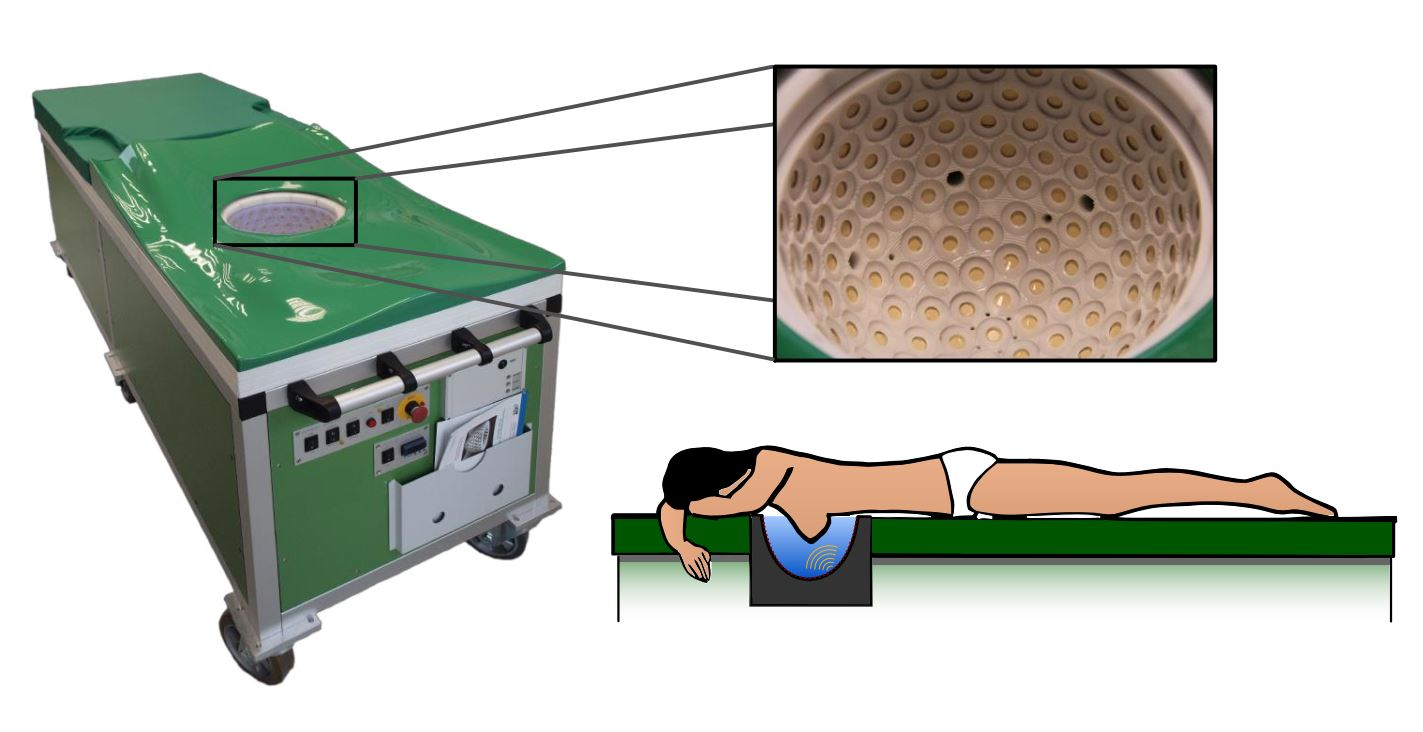
\includegraphics[width=1\textwidth]{usct_schematic.jpg}
    \caption{The prototype of an 3D-\ac{usct} device at the KIT research facility. Source: \cite{Kretzek2014GPUAberration}. }
    \label{usct_example}
\end{figure}


 The picture on the left shows the patient bed with the imaging aperture. The patients have to lie down on their stomach during the imaging procedure and have to remain as still as possible to avoid image degradation \cite{Ruiter2011RealizationUSCT}. One breast at a time will be placed in the water-filled semi-ellipsoidal imaging aperture. On the top-right of Figure \ref{usct_example} the aperture is shown with the ultrasound transducer elements mounted in the wall of the aperture.

To measure the pressure over time, the prototype of the \ac{usct} device at the KIT comprises 157 \acp{tas}. Each \ac{tas} consists of four emitting transducers and nine receiving transducers. Overall, 628 emitting and 1413 receiving transducers and ten aperture rotation positions are used to record \acp{ascan} to reconstruct an three dimensional images. Currently, ten positions are used, which was regarded as a good trade-off between the sparseness and the acquisition time. The aperture itself has a height of $17\,cm$ and diameter of $26\,cm$ \cite{Kretzek2014GPUAberration}.







\subsection{Multi-modality}
\label{sec:multimodality}

Three modalities for the reconstruction of a high resolution 3D-\ac{usct} image are currently in use: reflectivity, speed of sound and attenuation \cite{Jirik2012Sound-speedTomography}.

For the \textbf{Attenuation imaging} the \acp{ascan} of two transducers are compared. The sound wave interacts with the tissue and the coupling medium and loses intensity depending on the property of the tissue on that particular trajectory. The density of respective tissue influences the scattering and absorption of the sound waves energy. To quantify the attenuation a reference measurement of the empty imaging aperture precedes the actual acquisition of medical data. The amplitudes of the empty measurement are then compared to the levels with the breast in place. With an algebraic reconstruction technique the final attenuation-image can be reconstructed \cite{Dapp2011Geometry-independentInformation}. An example is given in Figure \ref{att_image_example}. The attenuation is given with the unit of attenuation in dB over the frequency of the ultrasound and the distance. The image shows the attenuation map of a breast phantom in the \ac{usct}. The bright spot in the middle is an artificial tumour. The brighter the colour of the tissue is depicted the higher is the attenuation of that part of the tissue.


\begin{figure}[H]
    \centering
    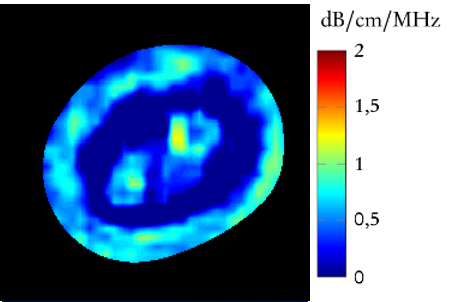
\includegraphics[width=0.55\textwidth]{Graphics/att_example.png}
    \caption{ Example of an attenuation image reconstructed by an algebraic reconstruction technique. }
    \label{att_image_example}
\end{figure}



\medskip

The \textbf{\ac{sos} imaging} technique is used to quantify the tissue specific sound speed. For that, the \acp{ascan} of  emitter-receiver-combinations are used for which the transducers are placed in the opposite site of the imaging aperture so that the sound waves have to pass through the tissue and the detected signals do not primarily arise from reflections. The comparison of the transmission pulse of the \ac{ascan} to the time of emission leads to a value for the propagation time and hence the \ac{sos} along the path from one transducer to the other. To get a 3D image the measurement has to be repeated for a multitude of emitter-receiver-combinations around the aperture. In \cite{Greenleaf1981ClinicalTomography} it was shown that with the \ac{usct} in transmission mode cysts in the female breast can be distinguished from surrounding tissue by the difference in sound speed in the different types of tissue. It was shown that normal tissue has a \ac{sos} of about $1400-1450 \, m/s$ and tumorous tissue a \ac{sos} of $1500 - 1520\, m/s$. Factors that influence the speed of sound in different types of tissue are the density, the micro-structure, temperature and elasticity of the tissue. Compared to the surrounding tissue the physical properties of tumours differ from the normal case and lead often to a higher speed of sound. 
Reconstructing the transmission image with an algebraic reconstruction technique helps classifying different tissue types by the means of their sound speed. An example for the same breast phantom as above is shown in Figure \ref{sos_image}. In this case the spot in the middle of the image shows a high speed of sound where the artificial tumour is located.

\begin{figure}[H]
    \centering
    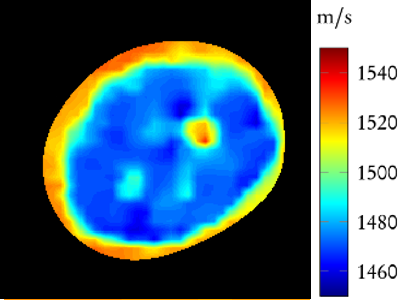
\includegraphics[width=0.50\textwidth]{Graphics/sos_example.png}
    \caption{ Example of a speed of sound map reconstructed by an algebraic reconstruction technique.}
    \label{sos_image}
\end{figure}


For the \textbf{Reflectivity imaging} technique one emitting transducer sends an ultrasound wave into the aperture and all receivers within an angle of approximately $0^{\circ} \, - \, 120^{\circ}$ between the sender normal and the receiver normal record the pressure over time. The measurement setup for one set of \acp{ascan} (i.e. for one emitter) can be seen in Figure \ref{measurement_volume}. Hence, not all receivers are used in this set of \acp{ascan}. The image shows the aperture from above with an tilted angle. All the active receivers are depicted in green for one emitter. On the opposite side of the group of emitters there is a gap where the \acp{ascan} of the receivers are not regarded. For the reflection imaging the values of these receivers have proven to lower the signal to noise ratio of the image and therefore are not regarded.


\begin{figure}[H]
    \centering
    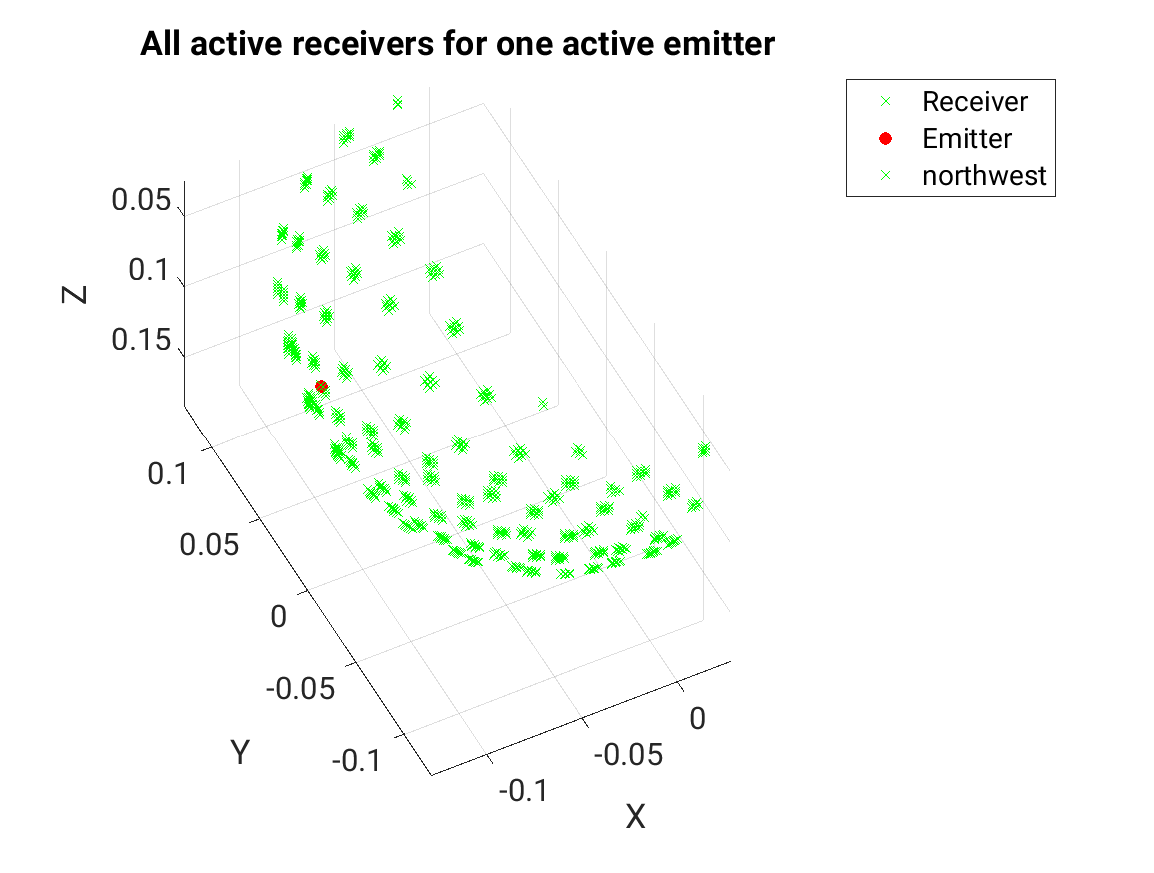
\includegraphics[width=0.75\textwidth]{Graphics/measurement_volume.eps}
    \caption{ The configuration of receivers for one active emitter. All used receivers are shown in green, the active emitter is plotted in red. The units are given in meters.}
    \label{measurement_volume}
\end{figure}

The breast phantom example for the reflection image is given in Figure \ref{reflecimage_example}. The resolution of the reflection image is much higher compared to the \ac{sos} map and the attenuation map. The information of the other two images can be combined to improve the resolution of the reflection image even further by providing information about local attenuation properties of the tissue as well as the sound speed can be regarded during the reconstruction of the reflection image.

\begin{figure}[H]
    \centering
    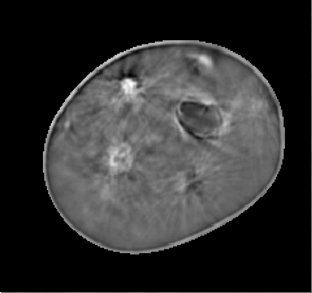
\includegraphics[width=0.55\textwidth]{Graphics/reflection_example.png}
    \caption{ Example of a reconstructed reflection image of the breast phantom.}
    \label{reflecimage_example}
\end{figure}
For the reconstruction of the reflection image the \ac{saft} is used. Since this thesis is mainly focused on the reconstruction of \ac{usct} reflection imaging the following section \ref{sec:SAFT} describes how \ac{saft} can be used to extract all the necessary information from the \acp{ascan} to reconstruct a high resolution reflection image. 






\subsection{Synthetic aperture focusing technique (SAFT)}
\label{sec:SAFT}
The \ac{saft} is used to reconstruct reflection images from the raw data of ultrasound imaging. By combining the data of the \acp{ascan} from a multitude of emitter-receiver combinations it is possible to reconstruct a high resolution image with sub-millimetre-resolution.

Figure \ref{ascan_example} shows the principle of an \ac{ascan}. The 3D volume of the aperture is shown on the left side. For this example only two of the many transducers that normally are placed on the wall of the aperture are shown. On the right the plot of the recorded \ac{ascan} at the receiver is shown by the graph. The actual \ac{ascan} consists of a discrete plot of the where the pressure $p(t)$ is plotted over the time $t$. The first pulse in the graph is the transmission pulse that reaches the receiving transducer. The second pulse originates from scattered waves at a certain location in the tissue and thus has a lower amplitude than the first pulse. The time duration it takes for the pulse to propagate from the emitter to the point of scattering and then to the receiving transducer is called \ac{tof}. One reason for the decreased amplitude of the reflected pulse compared to the transmission pulse is the longer path that the wave has to propagate. Scattering effects and reflections lead to the attnuation of the signal and therefore to a lower amplitude. 


\begin{figure}[H]
    \centering
    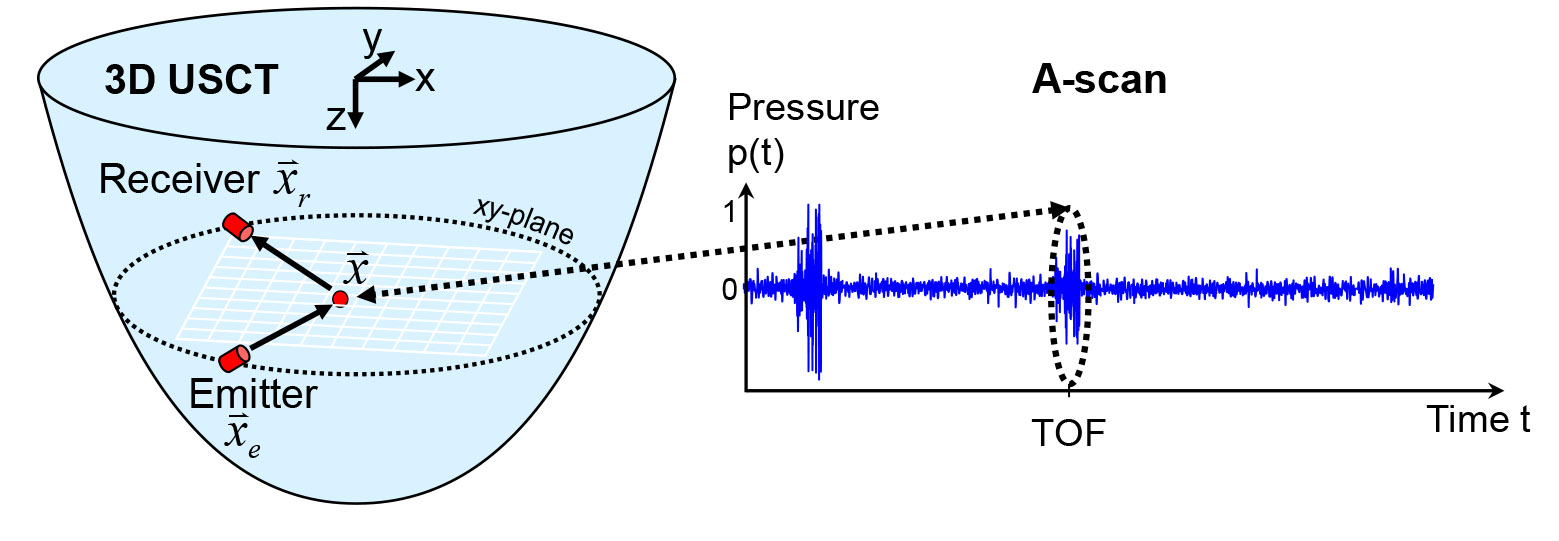
\includegraphics[width=1\textwidth]{GPU_based_3D_SAFT_reconstruction_including_phase_aberration-4.jpg}
    \caption{ Simple example of an \ac{ascan} for one emitter-receiver combination. One transducer $\overrightarrow{\chi_e}$ emits a pulsed wavefront into the aperture. The \ac{ascan} shows the pressure over the time measured by the receiving transducer $\overrightarrow{\chi_r}$. The first pulse in the diagram is the pulse cause by the direct transmission of the emitted wavefront. The second pulse is from the reflection of an object in the aperture. Source: \cite{Kretzek2014GPUAberration}. }
    \label{ascan_example}
\end{figure}

There are two principal ways to reconstruct an image from a set of \acp{ascan} using the \ac{saft} which both yield a similar result but differ in their computational cost. Each voxel eventually is assigned a certain value which corresponds to the intensity of that voxel in the final image. The intensity represents the echogenicity of the tissue at this particular position and is qualitatively proportional to the reflection coefficient.

\bigskip

For the \textbf{first method} one starts with the desired voxel that the value should be calculated for.
A simple 2D example of the xy-plane from Figure \ref{ascan_example} is shown in Figure \ref{SAFT_explain1}. On the left is the aperture with the 3D volume shown as a 2D grid. The emitter $\overrightarrow{{\chi_e }}$ and the two receiving transducers $\overrightarrow{{\chi_r }}$ and $\overrightarrow{{\chi_{r+1} }}$ are on the outer shell of the aperture. On the right two \acp{ascan} are depicted. The upper \ac{ascan} shows the plot of the pressure of the configuration where emitter $\overrightarrow{{\chi_e }}$ transmits a wavefront and $\overrightarrow{{\chi_r }}$ measures the transition of the pressure. The plot below is for emitter $\overrightarrow{{\chi_e }}$ but this time with transducer $r_{i+1}$ receiving. Considering how close $\overrightarrow{{\chi_r }}$ and $\overrightarrow{{\chi_{r+1} }}$ are placed to each other in this example the \ac{ascan} on the bottom shows an exaggerated negative time shift compared to the \ac{ascan} above.

\begin{figure}[H]
    \centering
    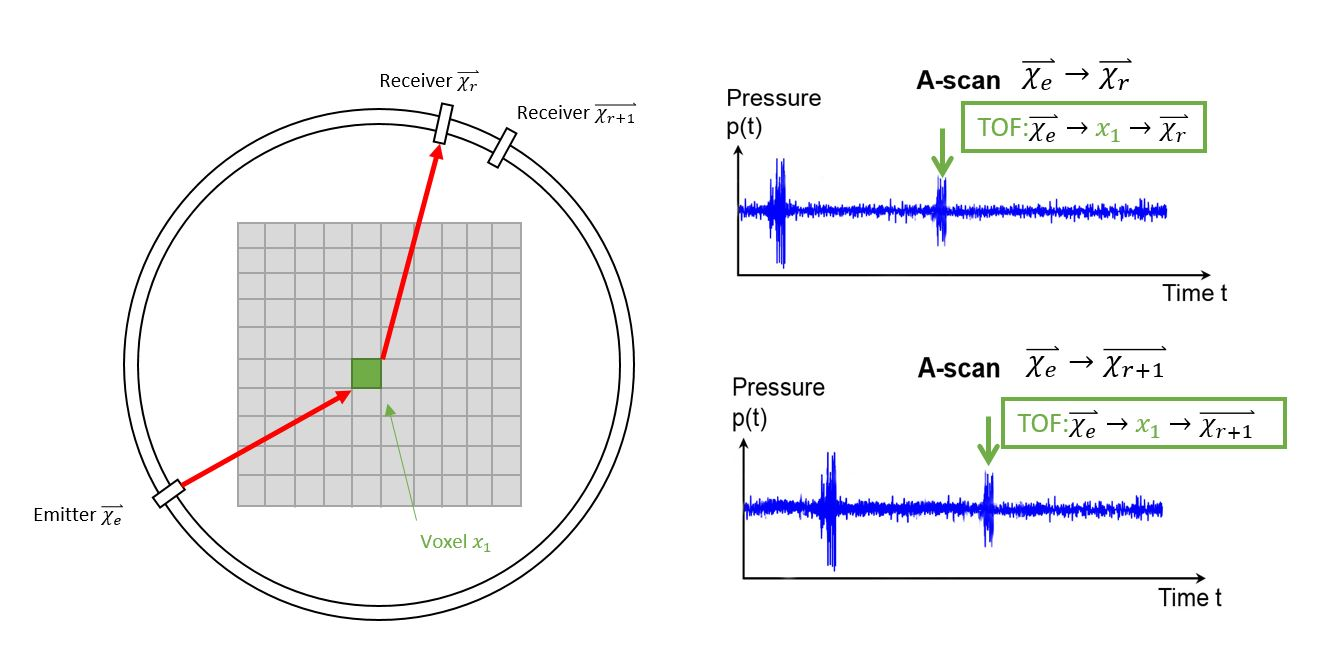
\includegraphics[width=1\textwidth]{SAFT_explaination1.jpg}
    \caption{Basic principle of the \ac{saft}. For one voxel every \ac{ascan} is analysed at a certain \ac{tof}. The final voxel value is the sum of every amplitude at the time in each corresponding \ac{ascan}. The procedure has to be repeated for each individual voxel. }
    \label{SAFT_explain1}
\end{figure}


For a known position of a voxel the \ac{tof} from each emitter to each receiving transducer can be calculated. For this basic example equation \ref{eqation_tof} shows how to calculate the \ac{tof} for the first voxel when neglecting the different speed of sound for the different types of tissue and assuming a constant \ac{sos}.

\begin{equation}
TOF_{1,ij} =  \frac{dist_{\overrightarrow{{\chi_e }},x_1} + dist_{x_1,\overrightarrow{{\chi_r }}} }{ SOS_{water} } 
\label{eqation_tof}
\end{equation}

$dist_{\overrightarrow{{\chi_e }},x_1}$ corresponds to the euclidean distance of the emitter $\overrightarrow{{\chi_e }}$ to the voxel $x_1$ and $dist_{x_1,\overrightarrow{{\chi_r }}}$ to the euclidean distance from the voxel $x_1$ to the receiver $\overrightarrow{{\chi_r }}$.
The speed of the sound wave is considered by $SOS_{water}$ in the equation.

The \ac{tof} for the first emitter-receiver combination is shown a the green arrow in the upper \ac{ascan} in Figure \ref{SAFT_explain1}. Here the \ac{tof} is directly located at the peak of the reflected wavefront. Since the \acp{ascan} have to be discretized the corresponding \ac{tof} may lay between two samples of the \ac{ascan}. To determine the appropriate value in the discrete set of samples either a linear 1D-interpolation between the two samples left and right of the \ac{tof} can be performed. Otherwise a nearest neighbour interpolation can yield a time sample.
For this \ac{tof} the amplitude of the \ac{ascan} then is taken and added to the voxel value of voxel $x_1$. 
In the same manner the \ac{tof} of the second receiver-emitter configuration is calculated and a sample in the \ac{ascan} can be found.
This procedure is repeated for every emitter-receiver combination and every aperture rotation shift so that the final result is the voxel value only for voxel $x_1$.
To reconstruct the whole 3D image these steps have to be repeated for every voxel in the volume.

Equation \ref{eqation_Voxel_value} shows the calculations necessary to get the voxel value $V_k$ for an arbitrary voxel $k$. 
\begin{equation}
V_k = \sum_{i}^{N_e}\sum_{j}^{N_r} A(TOF_{k,ij}) = \sum_{i}^{N_e}\sum_{j}^{N_r} A \left (\underset{ = TOF_{k,ij} } {\underbrace{\frac{ dist_{\overrightarrow{{\chi_e }},x_k} + dist_{x_k,\overrightarrow{{\chi_r }}}}{SOS_{water}} }}  \right )
\label{eqation_Voxel_value}
\end{equation}

For ${N_r}$ receiving and ${N_e}$ emitting transducers the reconstructed value $V$ of each voxel $k$ consists of the sum of all pressure values at the \ac{tof} in the respective \acp{ascan} for all emitter-receiver combinations ($N_e, N_r$). 

\bigskip
\bigskip

\begin{figure}[H]
    \centering
    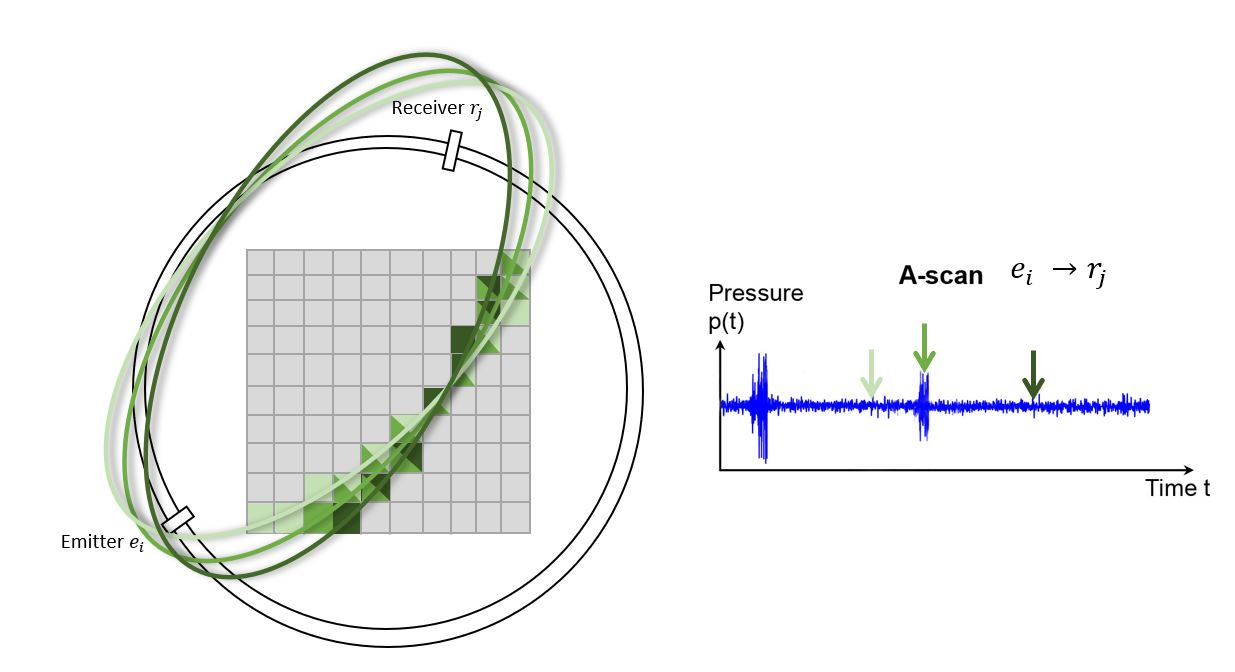
\includegraphics[width=1\textwidth]{SAFT_explaination2.jpg}
    \caption{ Alternative method to reconstruct the reflection image from the \acp{ascan}. }
    \label{SAFT_explain2}
\end{figure}


For the \textbf{second possibility} we do not start at a certain voxel but look at each individual \ac{ascan}. In Figure \ref{SAFT_explain2} the \ac{usct} aperture is shown this time with only one emitter-receiver configuration. On the right side the \ac{ascan} for this configuration is schematically plotted.
In contrast to the first method we do not only pick one certain sample in the \ac{ascan} but a few. In this example three samples are chosen marked by the arrows in the different shades of green. For each of the three chosen \acp{tof} there is one ellipse in Figure \ref{SAFT_explain2}. Along those ellipses, which is cut by the ellipse, the amplitude value of the \ac{ascan} is added to to the cut voxels. Bresenham's line drawing algorithm \cite{Bresenham2010AlgorithmPlotter} may be used to decide which set of voxels approximates the ellipse best and therefore to which voxel the corresponding amplitude value is added. An example is shown in Figure \ref{eclipse_super}.


%In contrast to the first method we do not only pick one certain sample in the \ac{ascan} but a few. 
%Theoretically one could use every sample in the \ac{ascan} to reconstruct the image, however is not recommendable as this would require a long time to compute. 

%In general it is advisable to pick at least one sample at location of the maximum peak that is caused by the scattering of the wavefront at the location of one voxel. In this example three samples are chosen marked by the arrows in the different shades of green. By choosing one sample in the \ac{ascan} we avoid having to 1D-interpolate during this step.

%With these three chosen \acp{tof} in one \ac{ascan} and the location of the emitter and receiver it is not possible to determine only one voxel to add the amplitude values to. For one emitter-receiver combination and one certain \ac{tof} a multitude of voxels are eligible to be the source of the scattering. To be precise an ellipse covers every possible scattering location where the \ac{tof} from emitter $\overrightarrow{{\chi_e }}$ to receiver $\overrightarrow{{\chi_r }}$ is equal to the chosen \ac{tof} from the \ac{ascan}. 

%For each of the three chosen \acp{tof} there is one ellipse in Figure \ref{SAFT_explain2}. Along those ellipses to every voxel, which is cut by the ellipse, the amplitude value is added to. This is schematically shown by the different shapes of the squares beneath each ellipse. A single colour means, that to that voxel only one value was added. Analogously do two or even three colours indicate, that multiple pressure values are added to that voxels value. 

%Bresenham's line drawing algorithm \cite{Bresenham2010AlgorithmPlotter} may be used to decide which set of voxels approximates the ellipse best and therefore to which voxel the corresponding amplitude value is added.

%This procedure leads to the fact, that many voxels get assigned pressure values even though they were not at the location of the scattering. However, when this procedure is repeated for every \ac{ascan} ultimately those voxels that are actually at the true location of the scattering will be part of so many ellipses that their final voxel value will be a lot higher than the surrounding noise. By superimposing the voxel values the surrounding noise is negligible and does not affect the final image. An example is shown in Figure \ref{eclipse_super}.

\begin{figure}[H]
    \centering
    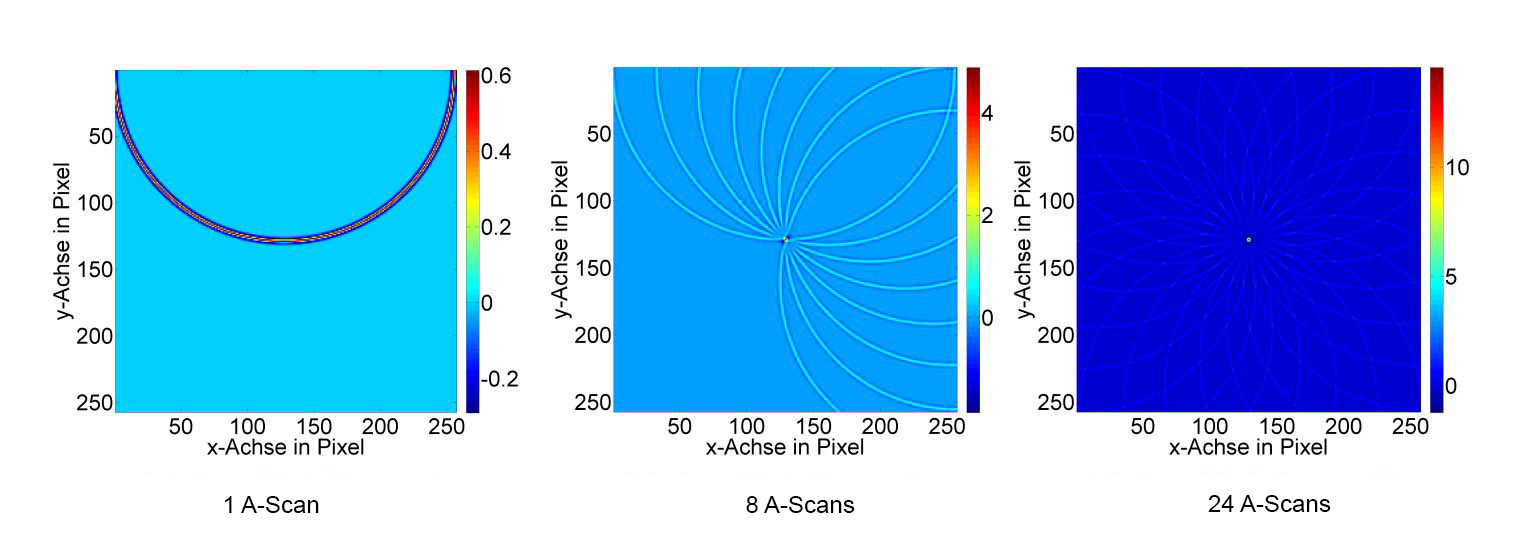
\includegraphics[width=1\textwidth]{eclipse_superposition_hucker.jpg}
    \caption{ Superposition of multiple ellipses during the reconstruction of the final image. By averaging the voxel values of multiple ellipses each ellipse loses significance in the final image.
    Source: \cite{PatrickHucker2014EvaluationRuckstreumodells}.}
    \label{eclipse_super}
\end{figure}

The example shows that the influence of each ellipse becomes less prominent with an increasing number of ellipses. Only at the point of scattering these ellipses superimpose and create a high amplitude that remains visible in the image.


%For only one \ac{ascan} the value of only that one \ac{tof} of the \ac{ascan} is added to each voxel along the ellipse. Therefore, the ellipse is very prominent in the left-most pane of Figure \ref{eclipse_super}. In the plot in the middle there are already eight different \acp{ascan} used. Each ellipse is still distinguishable but lost opacity nonetheless.
%In the pane on the right side 24 \acp{ascan} are superimposed. At the point of the intersection of all 24 ellipses one single pixel has a high value whereas the surrounding ellipses are barely visible anymore. The more \acp{ascan} are used for the reconstruction the higher the contrast of the final image gets.


Both methods have their advantages and disadvantages. However, during this thesis the first reconstruction algorithm was used. One of the main reasons for that is that all the calculations trivially be performed in parallel and therefore profit from the high number of threads of the GPU architecture. Furthermore, as was mentioned that the ellipse method makes multiple interpolations for each voxel in 3D necessary whereas the first method only interpolates in 1D between two sample values. By choosing the first method very expensive computation operations can be avoided.


\subsection{Speed of sound correction}
\label{sec:sos_correct}

For the \ac{saft} imaging there is no previous knowledge about the properties of the propagation speed in the medium. Until the \ac{sos} correction was introduced, for the \ac{saft} imaging, the propagation speed of the ultrasound was approximated to match the propagation speed of a sound wave in water: $SOS_{path} \approx  \bar{c}_{water}$  \cite{Kretzek2014GPUAberration}. The \ac{sos} was assumed to be constant for the whole path for the calculation of the \ac{tof} in each \ac{ascan} in this case. This assumption neglects the fact that the medium is not homogeneously filled with water. 

Since this is only a rough approximation of the actual \ac{sos} in the volume the assumption of a constant propagation speed led to a reduced contrast in the reconstructed image as the real location of the scattering was blurred during this process and small scatterers can not be resolved.
To improve the contrast of the final image for each path the \ac{sos} is calculated. With Bresenhams line drawing algorithm \cite{Bresenham2010AlgorithmPlotter} the appropriate voxels along the path from the emitter to the scattering voxel and further to the receiver are selected. For each of these $N$ visited voxels the local speed $c(\overrightarrow {x_k})$ is taken from the \ac{sos}-image from the preceding \ac{sos} measurement of the tissue.

The average speed of the sound propagation for that certain path $\overline{SOS}_{path}$ then can be calculated with the harmonic mean in equation \ref{path_sos} \cite{Kretzek2014GPUAberration}:

\begin{equation}
 \overline{SOS}_{path} = \frac{N}{\sum_{k=1}^{N}  \frac{1}{c(\overrightarrow {x_k})} } 
\label{path_sos}
\end{equation}

During the \ac{saft} in equation \ref{eqation_tof} and \ref{eqation_Voxel_value} the  $SOS_{water}$ can be replaced by the more realistic $\overline{SOS}_{path}$ for each individual propagation path.







\section{Characterisation of reflections}
\label{sig:flect_character}

During the acquisition of the data each emitting transducer emits a wavefront into the aperture which then interacts with the breast tissue in a distinct way. Therefore, it is important to take into consideration how the ultrasound wave interacts and scatters at the surface of the different tissue types and other objects in the aperture. The directional information of the reflections are lost during the classical approach of the \ac{saft} \cite{Kretzek2015EvaluationTomography}. As this thesis is focused on the tissue classification based on a back scattering model the reflection characteristics of the tissue can no longer be neglected. Figure \ref{fig:types_of_reflect} shows four different kinds of scattering and reflection depending on the structure of the surface and the direction of the incident ultrasound pulse.

\begin{figure}[H]
     \centering
     \begin{subfigure}[b]{0.23\textwidth}
         \centering
        \fbox{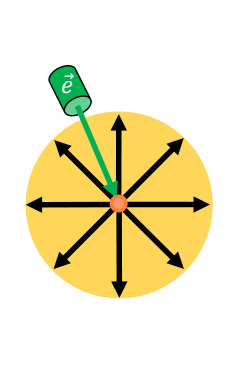
\includegraphics[width=0.8\linewidth]{ReflectionCharacteristics_IUS2015-1.jpg}}
         \caption{Isotropic scattering at point scatterer.}
         \label{fig:reflect_isotropic}
     \end{subfigure}
     \hfill
     \begin{subfigure}[b]{0.23\textwidth}
         \centering
         \fbox{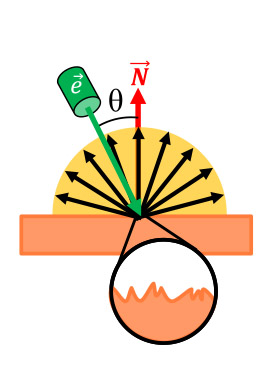
\includegraphics[width=0.87\textwidth]{ReflectionCharacteristics_IUS2015-2.jpg}}
         \caption{Diffuse scattering on rough surface.}
         \label{fig:reflect_diffuse}
     \end{subfigure}
     \hfill
     \begin{subfigure}[b]{0.23\textwidth}
         \centering
         \fbox{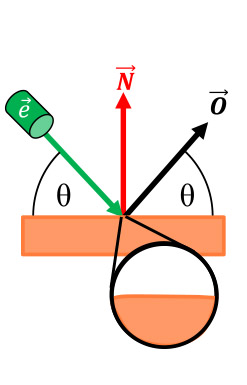
\includegraphics[width=0.8\textwidth]{ReflectionCharacteristics_IUS2015-3.jpg}}
         \caption{Specular reflection on a glossy surface.}
         \label{fig:reflect_specular}
     \end{subfigure}
     \hfill
     \begin{subfigure}[b]{0.23\textwidth}
         \centering
         \fbox{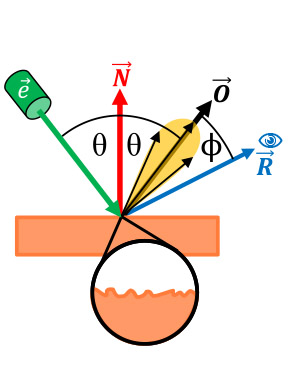
\includegraphics[width=0.93\textwidth]{ReflectionCharacteristics_IUS2015-4.jpg}}
         \caption{Specular reflection and diffuse reflection.}
         \label{fig:reflect_mixed}
     \end{subfigure}
        \caption{Reflection characteristics of different surfaces and angle of incidence. Source: \cite{Kretzek2015EvaluationTomography}}
        \label{fig:types_of_reflect}
\end{figure}


Figure \ref{fig:reflect_isotropic} shows the principle of isotropic scattering at a point scatterer. Transducer $\overrightarrow{e}$ emits a soundwave into the volume. When the sound wave reaches the point of scattering it will is reflected homogeneously into every direction with an isotropic distribution of intensity. This emitted spherical wave has a constant energy distribution in each direction. This is a theoretical principle of a reflection which the \ac{saft} is based on since it neglects all directional information of the received sound wave.

A better scattering model can be seen in figure \ref{fig:reflect_diffuse}. The diffuse scattering occurs on a rough and dull surface where the incoming energy of the ultrasound wave is equally scattered in every direction above the surface of the material (Lambertian reflectance). The surface of the material then appears to have the same radiance from every angle. The Lambert's Cosine Law states that the angle of the inciding wavefront has an influence on the radiated intensity \cite{lambert1892lamberts}.
The smaller the angle $\theta$ between the incoming wavefront and the surface normal $\overrightarrow{N}$, the larger the scattered intensity from the surface. In other words: the diffuse reflection is proportional to the amount of energy in form of ultrasound waves that hits the surface per unit area \cite{illum_Phong}, which is represented by equation \ref{eq:lambert_cosine}:

\begin{equation}
I_{diffuse} \propto cos(\theta)
\label{eq:lambert_cosine}
\end{equation}



\begin{figure}[H]
    \centering
    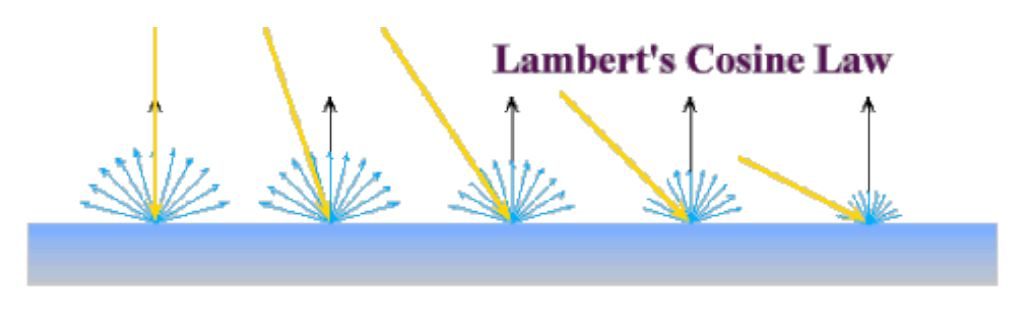
\includegraphics[width=0.75\textwidth]{lambert_cosine.jpg}
    \caption{Representation of the Lambert's Cosine Law. The scattered intensity from the surface is proportional to the cosine of the angle between the incoming wavefront and the surface normal. Source: \cite{illum_Phong}.}
    \label{Lambert_cosine_law}
\end{figure}


The third reflection characteristic is called specular reflection and can be seen in figure \ref{fig:reflect_specular}. Whereas in the case of the diffuse scattering the energy density of the scattered wave is evenly distributed above the surface facing the emitter, the specular reflection has a concentrated direction of emission. For glossy and even surfaces the incoming wave is reflected on the surface ideally whereas the entry angle  $\theta$ is equal to the exit angle $\theta$.
The main reflection direction is described by vector $\overrightarrow{o}$. For the ideal case of specular reflection the angle of the inciding soundwave equals the outgoing soundwave. Therefore the receiver normal has to be directly within the angle of the emitter normal to the surface. Otherwise the receiver would not detect any signal. 
%Furthermore, for an ideal specular reflection it is assumed that the energy of the incoming wavefront is equal to the reflected energy from the surface. 

%As the transducers of the 3D \ac{usct} emit unfocused ultrasound waves the angle of the incoming sound-wave can not be determined exactly. For the previous work \cite{PatrickHucker2014EvaluationRuckstreumodells} the specular reflection was assumed to be the prevailing model.


Figure \ref{fig:reflect_mixed} shows a combination of specular reflection and diffuse scattering. This model is appropriate for materials with a surface structure somewhere in-between rough and glossy. The emitted intensity is a mixture between the directly reflected energy based on the specular reflection and the scattered energy of the diffuse scattering model. This results in a cone shaped beam with an opening angle based on the scattering factor of the material. Again, the angle between the inciding wavefront and the surfaces normal determines the intensity of the reflected wave. Now also applies that the angle $\Phi$  between the receiver vector $\overrightarrow{R}$ to the main reflection direction $\overrightarrow{o}$ affects the received intensity as well. The smaller $\Phi$ becomes the greater is the measured intensity.








\section{Graphic processing unit (GPU)}

For the reconstruction of the image from the \acp{ascan} a sequence of calculations has to be performed which are highly parallelisable. In this section the benefits of utilizing \acp{gpu} to manage these calculations shall be addressed.

A main requirement for parallel calculations is that they can be performed independently from each other.
If there are certain dependencies between multiple simultaneous calculations so that one thread might have to wait on the intermediate result of the calculations of another thread then the whole process often becomes inefficient and unstable. 
In later chapters it will become clear that most of the calculations that are necessary for the reconstruction can be performed independently of each other. One example is the \ac{saft} during which for each voxel a certain value $V_k$ is determined. This process can be performed independently from the other voxels.
Beforehand, it was also mentioned that these processes of computation have to be repeated for each individual voxel. For a typical relevant volume of 1024x1024x1024 voxels this process can be parallelised for each individual voxel and profits from the \ac{gpu}s architecture. 

These kind of operations fall withing the scope of so-called \ac{simd}-operations. These \ac{simd}-operations are qualified by repeating the same or at least very similar operation on a changing set of data. Particularly, for this scenario \ac{gpu} are fitted with a high number of computation cores and high bandwidth memory buses.


\begin{figure}[H]
    \centering
    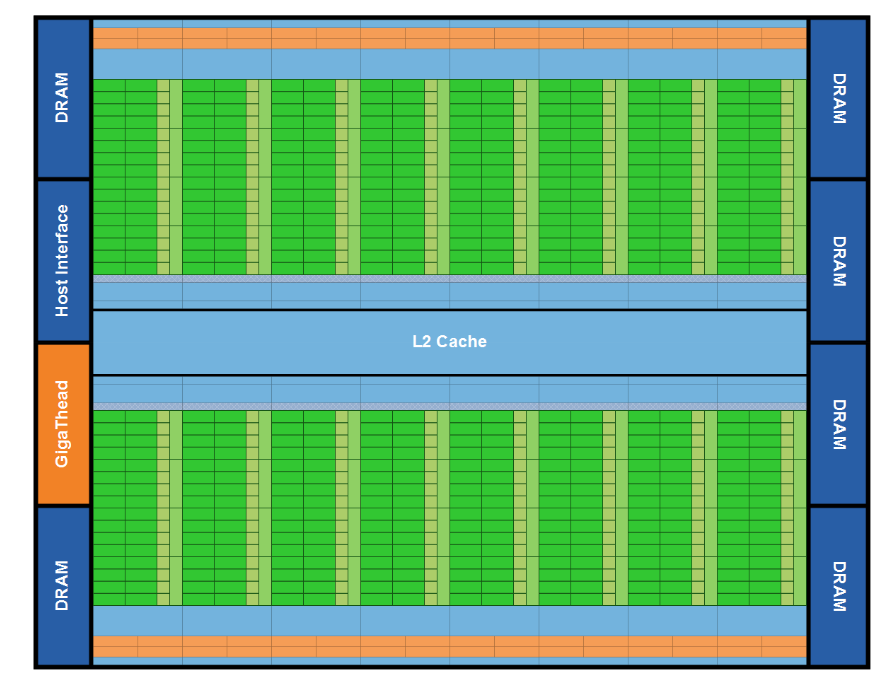
\includegraphics[width=0.75\textwidth]{Graphics/gpu_example.png}
    \caption{Example of a Fermi \ac{gpu} with 16 streaming modules(SM). Each SM is connected to the central Level 2 Cache which connects each core with each other. For each SM there are the 32 execution units coloured in green \cite{nvid_whitepaper}.}
    \label{nvidiea_aufbau}
\end{figure}


The current generation of RTX NVIDIA \acp{gpu} has up to 82 so-called \acp{sm} with a total of up to 10496 \acp{alu} \cite{gpu_stats}. These \acp{alu} are the unit of a processor which handles all operations which are necessary for the calculations. Simple arithmetic operations like for example additions and multiplications as well as logical operations like negation or AND-Conjunctions are managed by the \ac{alu}. The schematic of a basic \ac{gpu} architecture can be seen in Figure \ref{nvidiea_aufbau}. The schematic shows 16 \acp{sm} with 32 so-called CUDA-Cores each. The CUDA-Core represent the execution entities of the \ac{gpu}. Each \ac{sm} is connected to the Level 2 (L2) Cache which connects each \ac{sm} to the other. Furthermore, around those \acp{sm} there are units for storing larger amounts of data. The so-called DRAM, often also GDDR, is the random access memory of the \ac{gpu}. If enough \acp{gpu} are available it is possible to process large reconstruction volumes separately but in parallel and therefore minimise the memory access overhead when transferring data from the host to the device or vice versa.


In comparison a typical Intel i9 desktop central processing unit (CPU) in the 10\textsuperscript{th} generation has 10 physical and 20 logical processing units to work with \cite{intel_processor}. Besides the much higher number of processing units of the \ac{gpu} another big topic that is often overlooked is the memory bandwidth of the system. Of course, the number of \acp{alu} have a big impact in how fast each set of calculations can be finished. After finishing with the calculation the results have to be moved to the memory to wait for further processing. Often the bottle neck can be found in the data connection of the \acp{alu} to the host memory where ultimately every result is stored. Whereas the aforementioned Intel CPU has a memory bandwidth of 94 GB/s the NVIDIA \ac{gpu} profits of its 936 GB/s.
Furthermore, what makes \acp{gpu} so attractive for the reconstruction process of \ac{usct}-images is the hardware implemented texture unit. During the \ac{saft} there is the need for interpolating between two or more samples to find a feasible value for the \ac{ascan}. This operation can be done either in software or as a specialised hardware implementation which can process the data at a much higher speed. 


\subsection{CUDA-programming}
Besides having very powerful hardware at hand it is equally important to manage the data of the  reconstruction algorithm as efficiently as possible. With the introduction of the CUDA-programming technique NVIDIA made \ac{gpu}-programming much more accessible.
While the majority of code is written in C respectively C++ the actual core of the reconstruction is written in CUDA. The main objective of CUDA is to provide the programmer with a simple interface for her or his program components and get that particular software component to run on the \ac{gpu}. Some operations that are necessary before the code can be executed by the \ac{gpu} are for example the allocation of enough memory on the \ac{gpu}. Furthermore, the data has to be copied from the host computer to the CUDA-Device. The \ac{gpu} itself has no access to the RAM of the host machine. After that the CUDA-Kernel can be called. This is the central part of software that processes the raw data (in this case the \acp{ascan}) and yields the results of the calculation. 


\begin{figure}[H]
    \centering
    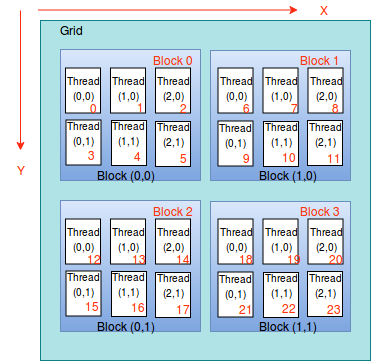
\includegraphics[width=0.55\textwidth]{Graphics/CudaIndexing.png}
    \caption{The organisation of threads when calling the kernel. Each thread is organised in blocks. These blocks again are substructures which are organised in grids \cite{cuda_indexing_guide}.}
    \label{cuda_index}
\end{figure}

When a CUDA-Kernel is called besides the main function there are two parameters that have to be set. These manage the indexing behaviour of the input data: the number of blocks per grid and the number of threads per block.
\begin{verbatim}
kernelFunction<<<numBlocks, threadsPerBlock>>>
\end{verbatim}
The indexing of a CUDA-Call can be seen in Figure \ref{cuda_index}. 
The parallel execution of a certain code segment leads to a new thread. Each thread serially numbered by the red numbers from 1 to 23 is organised in a 2D Block-Grid-Structure. The basic idea is that a certain number of threads can be organised into blocks. How many threads are summarised as a block can be managed by \begin{verbatim}
threadsPerBlock
\end{verbatim}
So the first 6 threads (0 - 5) are organised as the first Block 0. Each thread gets an internal ID the so-called  \begin{verbatim}
threadIdx
\end{verbatim}

The \code{threadIdx} is an up to 3D indexing-array to classify each thread running in each execution block. This can also be seen in Figure \ref{cuda_index} where each of the threads is indexed by a 2D vector.

A number of blocks then again can be summarised in a so-called grid. That is what the second parameter for the Kernel-Call is for:
With \begin{verbatim}
numBlocks
\end{verbatim}

Similar to the threads each block has a multi dimensional ID the so-called 
\begin{verbatim}
blockIdx
\end{verbatim}

An example is given in Figure \ref{blockidx_threadidx}:

\begin{figure}[H]
    \centering
    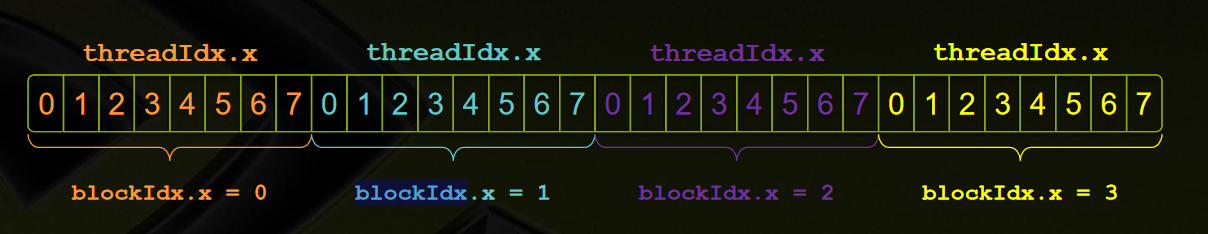
\includegraphics[width=0.89\textwidth]{Graphics/blockidxthreadix_explain.png}
    \caption{Example of how multiple, simultaneously executed threads are assigned to their \code{blockIdx}and \code{threadIdx}  \cite{cuda_indexing}.}
    \label{blockidx_threadidx}
\end{figure}

In this example there are each 8 threads per block. Their \code{threadIdx.x} are serially numbered from 0 to 7.
The first block is assigned \code{blockIdx.x = 0}. The \code{.x} indicates that in this case the \code{threadIdx} as well as the \code{blockIdx} are one dimensional and only have elements in x-direction. This process of numeration is repeated for all 32 threads so that every thread can be accessed by means of block-ID and thread-ID. Theoretically, these four blocks now can be  regarded as a grid.
A maximum of 1024 threads can be summarised as a block. A grid may contain up to 65535 blocks. Each block per grid then contains the same number of threads. The scheduling of all the threads onto the CUDA Cores is done by the CUDA Engine itself.
Furthermore, the parameters of the kernel call set how often the kernel function is called in total. In the kernel function the right set of data has to be picked depending on the \code{threadId} and the \code{blockId} so that the thread processes the right data.

